\documentclass[conference]{IEEEtran}
\IEEEoverridecommandlockouts
% The preceding line is only needed to identify funding in the first footnote. If that is unneeded, please comment it out.
\usepackage{cite}
\usepackage{amsmath,amssymb,amsfonts}
\usepackage{algorithmic}
\usepackage{graphicx}
\usepackage{textcomp}
\usepackage{romannum}
\usepackage{enumitem}   


\def\BibTeX{{\rm B\kern-.05em{\sc i\kern-.025em b}\kern-.08em
    T\kern-.1667em\lower.7ex\hbox{E}\kern-.125emX}}
\begin{document}

\title{CS6290: Reading Summary \Romannum{4}}

\author{\IEEEauthorblockN{Yang Ji}
\IEEEauthorblockA{ID:\ 56064832 \\
yangji@comp.hkbu.edu.hk \\
Dept.\ of Computer Science}
}

\maketitle

\section{Summary of Paper \cite{lu2018zebralancer}}

\subsection{Problem Statement}
This paper implements a crowdsourcing system atop public blockchain, namely ZebraLancer, which achieves the fair exchange without any trusted third party.
%
In particular, this system tries to resolve two general privacy challenges: (1) the tension between blockchain transparency and data confidentiality (2) the tension between anonymity and accountability. 

\subsection{Problem Significance}
In practice, the reduction of the reliance on a trusted third-party is desirable due to the following reasons:
%
\begin{itemize}
    \item The arbiter might misbehave for his/her own self-interets. 
    \item Current crowdsourcing systems are biased on requestors over workers.
    \item Single point failure.
    \item Massive privacy leakage. For example, Uber tried to hide the fact of data leakage in 2016.  
\end{itemize}
 
\subsection{Preliminaries}
\subsubsection{Crowdsourcing System}
Crowdsourcing is a common business model which empowers open and wide collaboration over the Internet with lower cost and high scalability.
%
In the standard crowdsourcing system, requesters need to adopt reasonable incentive policies to encourage workers' participation.
%
To ensure the fair exchange, a trusted third party is usually used to host crowdsourcing tasks and help resolve the dispute.
%

\subsection{State of the Art}
To solve the above problems, we could employ open blockchains to remove a trusted third-party and realize a decentralized crowdsourcing system.
%
Blockchain has many valuable features which can help remove the trusted arbiter safely. 
%
Firstly, open blockchain could be viewed as a distributed, transparent and immutable public 'bulletin board'.
%
Any data can't be modified and accessible to the public.
%
Then pre-defined consensus protocol ensures reliable message deliveries via the untrusted Internet. 
%
What's more, smart contract can faithfully execute all computations and message deliveries.
%
Requesters can deploy tasks in the form of smart contract into the blockchain and workers can submit their answers to the corresponding addresses through transactions.

However, public blockchain also brings about many new problems which are not shown before at all.
%
For one thing, transparency violates data privacy directly.
%
For example, workers' submitted answers are exposed to other peers who can simply copy them and form free-riding attacks.
%
For another thing, totally transparency could cause misbehaviors by colluded counterfeit identities.

\begin{figure}[ht]
    \centering
    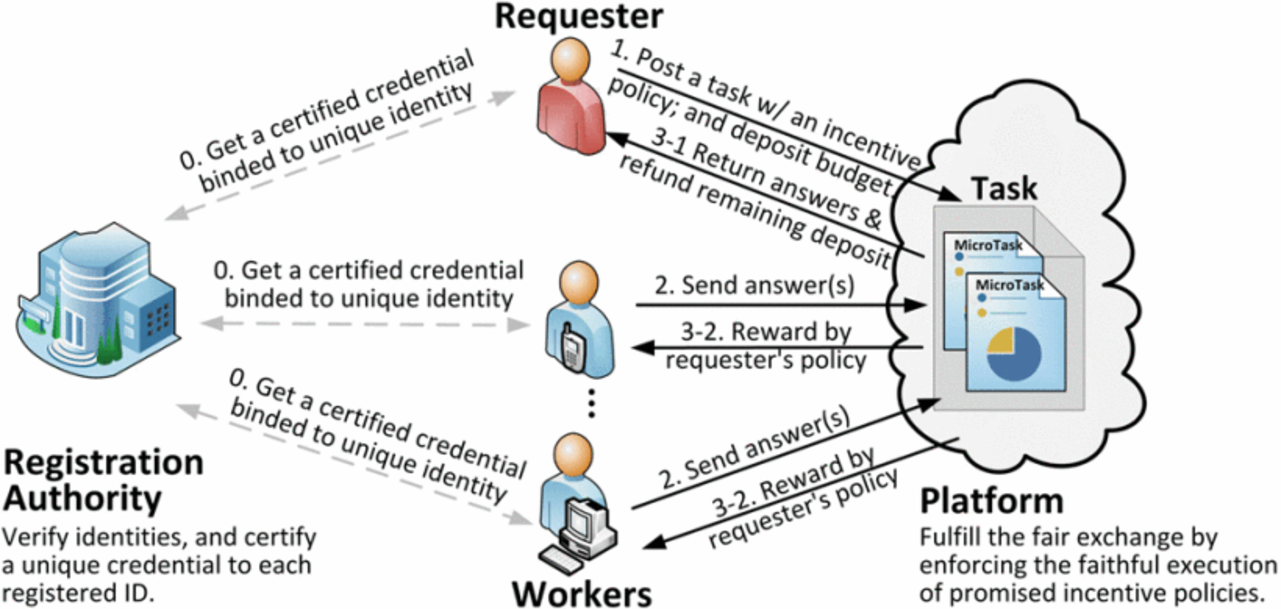
\includegraphics[width= 0.95\linewidth]{fig/system1.pdf}
    \caption{Model of decentralized crowdsourcing system}
    \label{arch}
\end{figure}

\subsection{Contributions}
The model of data crowdsourcing consists of four components:
\begin{itemize}
    \item \textbf{Registration Authority (RA).} All users including requesters and workers must obtain unique credentials from RA which are bound to their true identities.
    \item \textbf{Authenticated Requesters.} Users who issue crowdsourcing tasks.
    \item \textbf{Authenticated Workers.} Users who help resolve launched tasks.
    \item \textbf{Platform.} This platform is used to fulfill the fair exchange by faithfully executing requesters' pre-defined incentive policies. In this paper, this platform is actually Ethereum. 
\end{itemize} 

It is worth nothing that RA is introduced to prevent users from misusing anonymity. 
%
The authors define existing problems of decentralized crowdsourcing systems as follows: 
(1) \textbf{Data Confidentiality:} Any information of the content of submitted answers shouldn't be accessible to the public.  
(2) \textbf{Anonymity:} This property ensures that we can't link a submission or joined tasks to a particular worker/requester.

To settle the first treat, the authors enforce the workers to encrypt their submitted answers under the requester's public key, which means only the requester of this task could decrypt these answers.
%
But this leads to a new problem for smart contract because encryption prevents smart contract from executing the incentive policy and requesters can't put their secret keys on the smart contract directly.
%
In this paper, the authors leverage a zero-knowledge cryptographic tool called zk-SNARK to realize a proving and verifying mechanism to guarantee the fairness in exchange.
%
In more detail, the requester needs to generate a zero-knowledge proof of his/her faithful computation and smart contract could verify this succinct proof expediently.

For the second security issue, the authors create a common-prefix-linkable anonymous authentication scheme to keep sure that users could submit anonymous answers once for one task.
%
Once a particular worker submits his/her answer more than once, smart contract can link these submissions together, which could prevent the misuse of anonymity efficiently.
%
The detailed solution is to append a prefix string to each submission which corresponds to each task.

\subsection{Remaining Questions}
Firstly, I think requesters don't need to hash their secret keys in the head which seems redundant in the whole scheme construction.
%
Secondly, the experiment results show that incentive policy is quite simple which only costs 10ms for verification.
%
Thirdly, zk-SNARK needs a trusted setup phase to generate proving and verifying key ,which means more dependencies on Registration Authority.


\section{Summary of Paper\cite{tramer2017sealed}}

\subsection{Problem Statement}
Recent years have witnessed an unprecedented increase in applications of trusted hardware systems like Intel Software Guard extension (SGX).
%
SGX is designed to ensure the faithful execution and data confidentiality of user-level codes through hardware protection.
%
Recent studies, however, raise the widespread concerns of the security of SGX.
%
Since there exist some resources which are shared between enclaves and untrusted hosts, the perfect isolation is broken causing by various side channel attacks.

Based on this background, the authors aim to find possible applications in practice using SGX without any confidentiality requirement.

\subsection{Problem Significance}
Emerging attacks on state confidentiality of SGX make the original security requirement challenging.
%
And it seems that there are no efficient attacks working on the faithful execution of programs inside enclaves.
%
For the first in the literature, the authors propose the model called \textsl{transparent enclave execution}, wherein computational integrity is guaranteed without data confidentiality.
%
What's more, they also explore what functionality could be realized atop it.


\subsection{Preliminaries}
In this part, I briefly recap the basic functions and principles of Intel SGX.
%
As aforementioned, SGX enables the creation of "isolated software enclaves" which are designed for providing the confidentiality, integrity and authenticity of program execution even when operating systems are compromised.

In general, SGX allows remote entities to verify its generated attestation which proves the secure running of the programs in the enclave.
%
When first initialized, the CPU would generate a hash of the original state, namely \textsl{measurement}.
%
Then SGX uses its physically protected key, and a group signature scheme named \textsl{Enhanced Privacy ID} to produce a corresponding attestation.
%
Remote entities could get to know that the measured software is indeed running in SGX-protected enclaves.

\begin{figure}[ht]
    \centering
    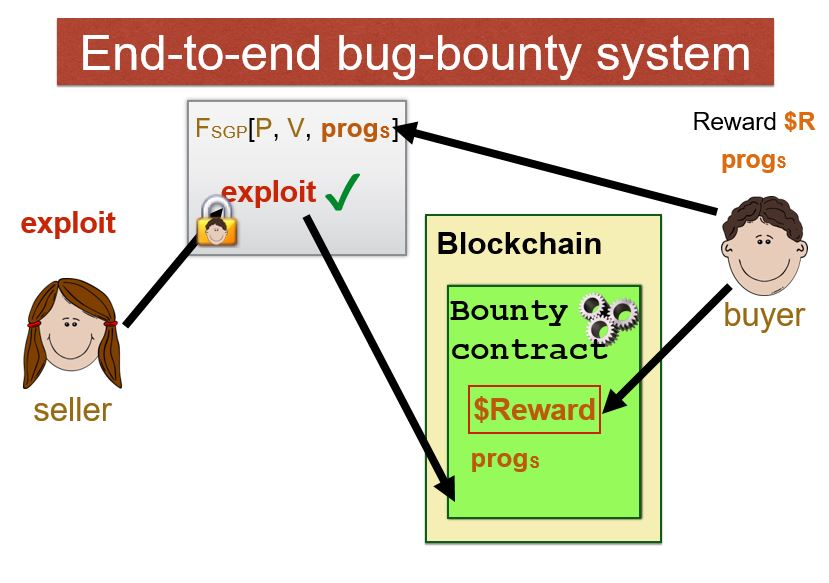
\includegraphics[width= 0.95\linewidth]{fig/system2.jpg}
    \caption{End-to-end bug-bounty system}
    \label{e2e}
\end{figure}

\subsection{State of the Art}
No previous works do with SGX without confidentiality.

As for verifiable computation and zero-knowledge proofs, many advances, like zk-SNARKs\cite{ben2013snarks} and garbled circuits\cite{huang2011faster}, have been achieved recently.
%
Compared to this transparent enclave, these methods only support limited programs to be transformed into polynomials in the form of quadratic arithmetic programs.

In the knowledge marketplace, "Zero-Knowledge Contingent Protocol" is proposed to realize the fair exchange between knowledge and rewards by using blockchain.
%
Basic procedures could be described as follows:
\begin{itemize}
    \item \textit{Public predicate:} Buyer publishes a transaction to collect targeted answers from the public.
    \item \textit{Create offer:} Seller then generates and sends a tuple offer$(\pi,h,c)$, where $\pi$ means a zk-proof of correct answers, $h$ denotes the hash of secret key $k$ and $c$ represents the encryption of input answers under $k$.
    \item \textit{Post conditional transactions:} After verifying the correctness of the tuple, buyer could send a \textit{hashlock} function to the blockchain.
    \item \textit{Claim reward:} Using the real key, seller could obtain his/her rewards.
    \item \textit{Recover up:} Last, seller could use this secret key to decrypt the previous answer.
\end{itemize}

The authors mainly argue that zk arguments are prohibitively constructed and become impractical in the real marketplace.
%
What's more, buyer could still cancel the transaction after knowing the existence of the answer (might be a bug in the software). 

\subsection{Contributions}
In this work, the authors aim at realizing a strong proof system called sealed-glass proof (SGP) which can be used to generalize ZK proofs, commitment schemes and verifiable computing.
%
This transparent enclaves could be deployed securely in the system model wherein parties are untrusted to each other and have inherent resource asymmetry.

Here, I take bug bounty platform like the SQL injection as an example.
%
In this case, the program should randomly initialize a user database for sellers and check whether they could use exploits to login in this database.
%
The first problem is that since the enclave is totally transparent, finding an exploit is very trivial if the whole database is first deployed.
%
Therefore, sellers should provide the knowledge of exploit by using commitment before the database is populated.
%
By using SGP, we can realize the proof of the knowledge.

Another building block is about how to realize the fair exchange between sellers and buyers.
%
As has been discussed in the state-of-the-art part, ZKCP protocol could not be employed directly here.
%
This paper mainly propose an end-to-end bug-bounty system wherein SGP is running between the seller and the contract.
%
The system architecture is described in Figure\ref{e2e}.
%
It is worth nothing that we can't run the smart contract directly since its state is totally transparent.
%
On the contrary, smart contract could verify the attestation and send pre-defined rewards faithfully.
%
Through encrypting answers under buyer's public key, this system also achieves data confidentiality at the same time.

\subsection{Remaining Questions}
This paper doesn't target on the complexity of reward policies in the real knowledge marketplace.
%
Whether this proposition could support more complicated reward policy still remains a question. 

\bibliographystyle{IEEEtran}
\bibliography{references}


\end{document}
